\documentclass[11pt,a4paper]{report}
\usepackage[textwidth=37em,vmargin=30mm]{geometry}
\usepackage{calc,xunicode,amsmath,amssymb,paralist,enumitem,tabu,booktabs,datetime2,xeCJK,xeCJKfntef,listings}
\usepackage{tocloft,fancyhdr,tcolorbox,xcolor,graphicx,eso-pic,xltxtra,xelatexemoji}

\newcommand{\envyear}[0]{2025}
\newcommand{\envdatestr}[0]{2025-09-04}
\newcommand{\envfinaldir}[0]{webdb/2025/20250904/final}

\usepackage[hidelinks]{hyperref}
\hypersetup{
    colorlinks=false,
    pdfpagemode=FullScreen,
    pdftitle={Web Digest - \envdatestr}
}

\setlength{\cftbeforechapskip}{10pt}
\renewcommand{\cftchapfont}{\rmfamily\bfseries\large\raggedright}
\setlength{\cftbeforesecskip}{2pt}
\renewcommand{\cftsecfont}{\sffamily\small\raggedright}

\setdefaultleftmargin{2em}{2em}{1em}{1em}{1em}{1em}

\usepackage{xeCJK,xeCJKfntef}
\xeCJKsetup{PunctStyle=plain,RubberPunctSkip=false,CJKglue=\strut\hskip 0pt plus 0.1em minus 0.05em,CJKecglue=\strut\hskip 0.22em plus 0.2em}
\XeTeXlinebreaklocale "zh"
\XeTeXlinebreakskip = 0pt


\setmainfont{Brygada 1918}
\setromanfont{Brygada 1918}
\setsansfont{IBM Plex Sans}
\setmonofont{JetBrains Mono NL}
\setCJKmainfont{Noto Serif CJK SC}
\setCJKromanfont{Noto Serif CJK SC}
\setCJKsansfont{Noto Sans CJK SC}
\setCJKmonofont{Noto Sans CJK SC}

\setlength{\parindent}{0pt}
\setlength{\parskip}{8pt}
\linespread{1.15}

\lstset{
	basicstyle=\ttfamily\footnotesize,
	numbersep=5pt,
	backgroundcolor=\color{black!5},
	showspaces=false,
	showstringspaces=false,
	showtabs=false,
	tabsize=2,
	captionpos=b,
	breaklines=true,
	breakatwhitespace=true,
	breakautoindent=true,
	linewidth=\textwidth
}






\newcommand{\coverpic}[2]{
    % argv: itemurl, authorname
    Cover photo by #2~~(\href{#1}{#1})
}
\newcommand{\makeheader}[0]{
    \begin{titlepage}
        % \newgeometry{hmargin=15mm,tmargin=21mm,bmargin=12mm}
        \begin{center}
            
            \rmfamily\scshape
            \fontspec{BaskervilleF}
            \fontspec{Old Standard}
            \fontsize{59pt}{70pt}\selectfont
            WEB\hfill DIGEST
            
            \vfill
            % \vskip 30pt
            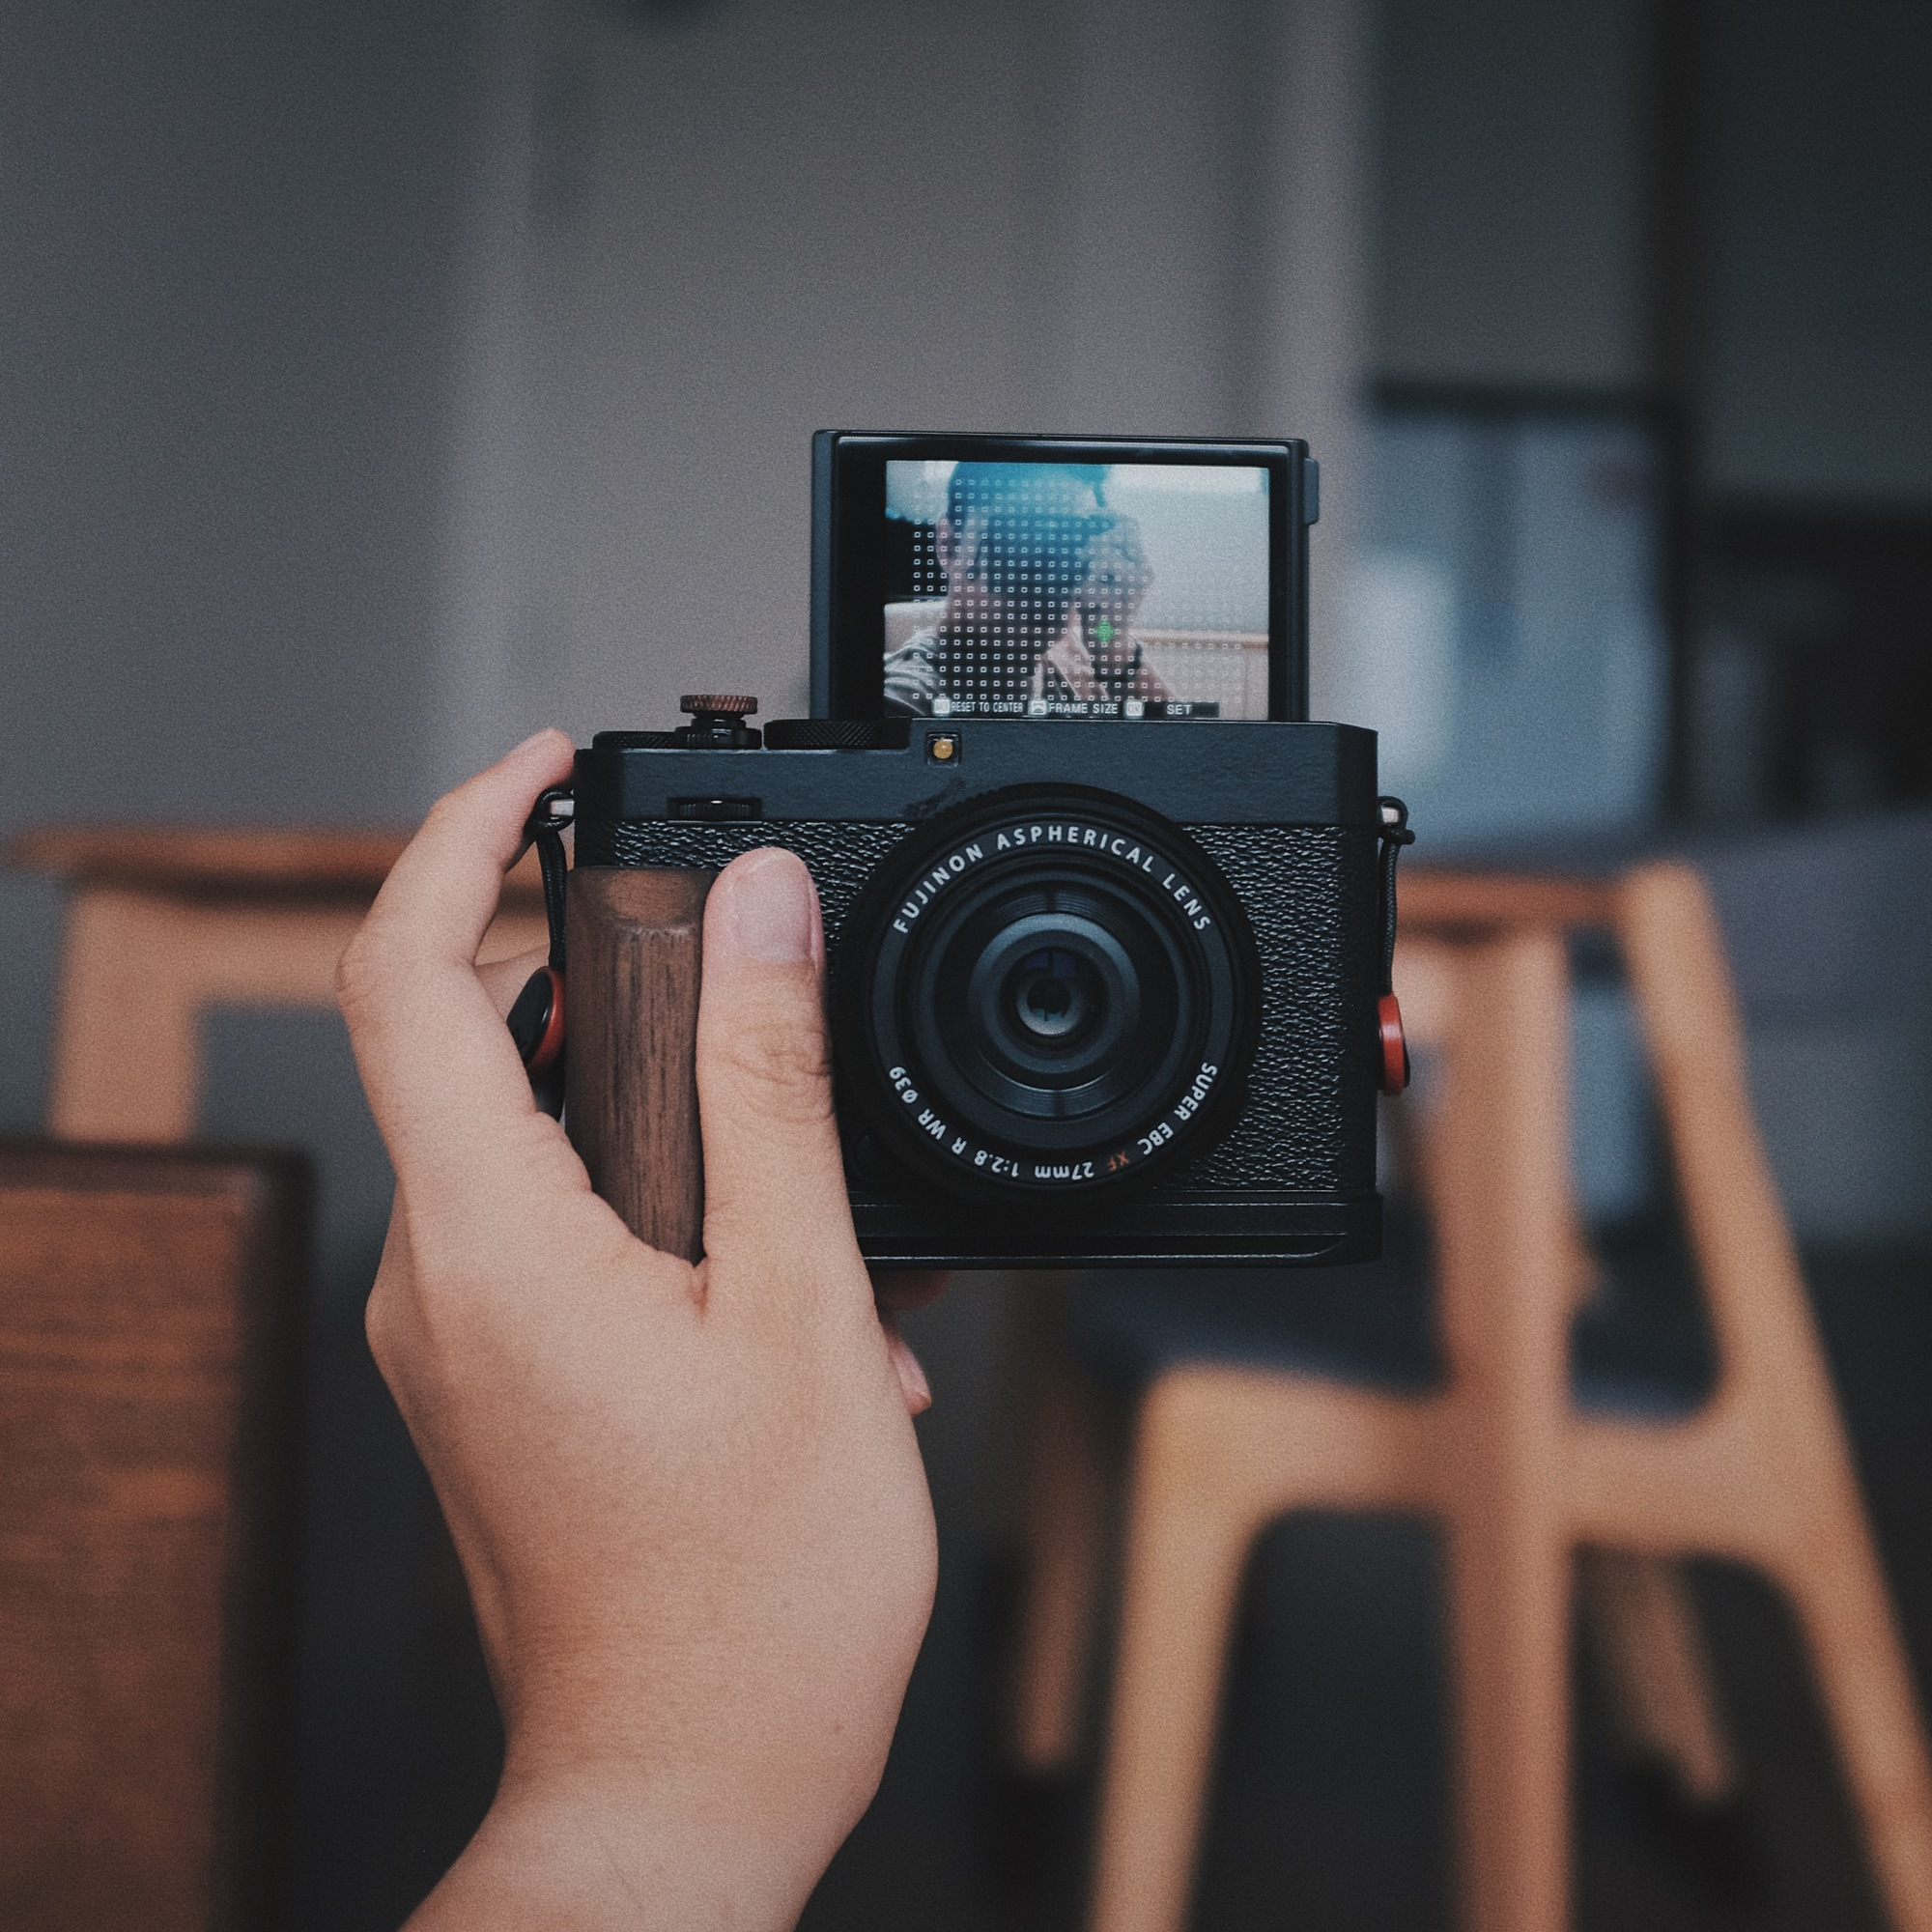
\includegraphics[width=\linewidth]{\envfinaldir/coverpic-prod.jpg}\par
            % \vskip 30pt
            \vfill

            \normalsize\rmfamily\scshape
            \copyright{} The Web Digest Project \hfill\large \envdatestr
        \end{center}
    \end{titlepage}
    % \restoregeometry
}
\newcommand{\simplehref}[1]{%
    \textcolor{blue!80!green}{\href{#1}{#1}}%
}
\renewcommand{\contentsname}{\center\Huge\sffamily\bfseries Contents\par\vskip 20pt}
\newcounter{ipartcounter}
\setcounter{ipartcounter}{0}
\newcommand{\ipart}[1]{
    % \vskip 20pt
    \clearpage
    \stepcounter{ipartcounter}
    \phantomsection
    \addcontentsline{toc}{chapter}{#1}
    % \begin{center}
    %     \Huge
    %     \sffamily\bfseries
    %     #1
    % \end{center}
    % \vskip 20pt plus 7pt
}
\newcounter{ichaptercounter}
\setcounter{ichaptercounter}{0}
\newcommand{\ichapter}[1]{
    % \vskip 20pt
    \clearpage
    \stepcounter{ichaptercounter}
    \phantomsection
    \addcontentsline{toc}{section}{\numberline{\arabic{ichaptercounter}}#1}
    \begin{center}
        \Huge
        \sffamily\bfseries
        #1
    \end{center}
    \vskip 20pt plus 7pt
}
\newcommand{\entrytitlefont}[1]{\subsection*{\raggedright\Large\sffamily\bfseries#1}}
\newcommand{\entryitemGeneric}[2]{
    % argv: title, url
    \parbox{\linewidth}{
        \entrytitlefont{#1}\par\vskip 5pt
        \footnotesize\ttfamily\mdseries
        \simplehref{#2}
    }\vskip 11pt plus 11pt minus 1pt
}
\newcommand{\entryitemGithub}[3]{
    % argv: title, url, desc
    \parbox{\linewidth}{
        \entrytitlefont{#1}\par\vskip 5pt
        \footnotesize\ttfamily\mdseries
        \simplehref{#2}\par\vskip 5pt
        \small\rmfamily\mdseries#3
    }\vskip 11pt plus 11pt minus 1pt
}
\newcommand{\entryitemAp}[3]{
    % argv: title, url, desc
    \parbox{\linewidth}{
        \entrytitlefont{#1}\par\vskip 5pt
        \footnotesize\ttfamily\mdseries
        \simplehref{#2}\par\vskip 5pt
        \small\rmfamily\mdseries#3
    }\vskip 11pt plus 11pt minus 1pt
}
\newcommand{\entryitemHackernews}[3]{
    % argv: title, hnurl, rawurl
    % \parbox{\linewidth}{
    %     \entrytitlefont{#1}\par\vskip 5pt
    %     \footnotesize\ttfamily\mdseries
    %     \simplehref{#3}\par
    %     \textcolor{black!50}{\href{#2}{#2}}
    % }\vskip 11pt plus 11pt minus 1pt
    \begin{minipage}{\linewidth}
            \entrytitlefont{#1}\par\vskip 5pt
            \footnotesize\ttfamily\mdseries
            \simplehref{#3}\par
            \textcolor{black!50}{\href{#2}{#2}}
    \end{minipage}\par\vskip 11pt plus 11pt minus 1pt
}







\begin{document}

\makeheader

\tableofcontents\clearpage




\ipart{Developers}
\ichapter{Hacker News}
\entryitemTwoLinks{Where's the shovelware? Why AI coding claims don't add up}{https://news.ycombinator.com/item?id=45120517}{https://mikelovesrobots.substack.com/p/wheres-the-shovelware-why-ai-coding}

\entryitemTwoLinks{The worst possible antitrust outcome}{https://news.ycombinator.com/item?id=45120050}{https://pluralistic.net/2025/09/03/unpunishing-process/}

\entryitemTwoLinks{Tufte CSS}{https://news.ycombinator.com/item?id=45119103}{https://edwardtufte.github.io/tufte-css/}

\entryitemTwoLinks{We're Joining OpenAI}{https://news.ycombinator.com/item?id=45119076}{https://www.alexcodes.app/blog/alex-team-joins-openai}

\entryitemTwoLinks{What is it like to be a bat?}{https://news.ycombinator.com/item?id=45118592}{https://en.wikipedia.org/wiki/What\_Is\_It\_Like\_to\_Be\_a\_Bat\%3F}

\entryitemTwoLinks{Poor man's bitemporal data system in SQLite and Clojure}{https://news.ycombinator.com/item?id=45118585}{https://www.evalapply.org/posts/poor-mans-time-oriented-data-system/index.html}

\entryitemTwoLinks{Microsoft BASIC for 6502 Microprocessor – Version 1.1}{https://news.ycombinator.com/item?id=45118392}{https://github.com/microsoft/BASIC-M6502}

\entryitemTwoLinks{Speeding up PyTorch inference on Apple devices with AI-generated Metal kernels}{https://news.ycombinator.com/item?id=45118111}{https://gimletlabs.ai/blog/ai-generated-metal-kernels}

\entryitemTwoLinks{Who Owns, Operates, and Develops Your VPN Matters}{https://news.ycombinator.com/item?id=45117974}{https://www.opentech.fund/news/who-owns-operates-and-develops-your-vpn-matters-an-analysis-of-transparency-vs-anonymity-in-the-vpn-ecosystem-and-implications-for-users/}

\entryitemTwoLinks{Writing a C compiler in 500 lines of Python (2023)}{https://news.ycombinator.com/item?id=45117668}{https://vgel.me/posts/c500/}

\entryitemTwoLinks{Nuclear: Desktop music player focused on streaming from free sources}{https://news.ycombinator.com/item?id=45117230}{https://github.com/nukeop/nuclear}

\entryitemTwoLinks{Understanding Transformers Using a Minimal Example}{https://news.ycombinator.com/item?id=45116957}{https://rti.github.io/gptvis/}

\entryitemTwoLinks{Claude Code: Now in Beta in Zed}{https://news.ycombinator.com/item?id=45116688}{https://zed.dev/blog/claude-code-via-acp}

\entryitemTwoLinks{Airbus B612 Cockpit Font}{https://news.ycombinator.com/item?id=45115942}{https://github.com/polarsys/b612}

\entryitemTwoLinks{Building the most accurate DIY CNC lathe in the world [video]}{https://news.ycombinator.com/item?id=45115760}{https://www.youtube.com/watch?v=vEr2CJruwEM}

\entryitemTwoLinks{For all that's holy, can you just leverage the Web, please?}{https://news.ycombinator.com/item?id=45115550}{https://blog.tomayac.com/2025/09/03/for-all-thats-holy-can-you-just-leverage-the-web-please/}

\entryitemTwoLinks{John Coltrane's Tone Circle}{https://news.ycombinator.com/item?id=45115004}{https://roelsworld.eu/blog-saxophone/coltrane-tone-circle/}

\entryitemTwoLinks{MIT Study Finds AI Use Reprograms the Brain, Leading to Cognitive Decline}{https://news.ycombinator.com/item?id=45114753}{https://publichealthpolicyjournal.com/mit-study-finds-artificial-intelligence-use-reprograms-the-brain-leading-to-cognitive-decline/}

\entryitemTwoLinks{Voyager – An interactive video generation model with realtime 3D reconstruction}{https://news.ycombinator.com/item?id=45114379}{https://github.com/Tencent-Hunyuan/HunyuanWorld-Voyager}

\entryitemTwoLinks{UK Electricity Generation Map}{https://news.ycombinator.com/item?id=45114277}{https://www.energydashboard.co.uk/map}


\ipart{Developers~~~~(zh-Hans)}
\ichapter{Solidot}
\entryitemGeneric{\hskip 0pt{}Google 允许保留 Chrome 但被禁止签订独占搜索引擎交易}{https://www.solidot.org/story?sid=82210}

\entryitemGeneric{\hskip 0pt{}特斯拉在华销量连续两个月下滑,马斯克称人形机器人是公司未来}{https://www.solidot.org/story?sid=82209}

\entryitemGeneric{\hskip 0pt{}美国 85\% 的大学生报告使用 AI 完成作业 }{https://www.solidot.org/story?sid=82208}

\entryitemGeneric{\hskip 0pt{}联合国报告称深圳-香港-广州是全球第一大创新集群}{https://www.solidot.org/story?sid=82207}

\entryitemGeneric{\hskip 0pt{}2025 年可能是美国有记录以来人口首次减少的一年}{https://www.solidot.org/story?sid=82206}

\entryitemGeneric{\hskip 0pt{}烟灰行星可能比水世界更常见}{https://www.solidot.org/story?sid=82205}

\entryitemGeneric{\hskip 0pt{}资深程序员比初级程序员更可能使用 AI 生成代码}{https://www.solidot.org/story?sid=82204}

\entryitemGeneric{\hskip 0pt{}GNOME 基金会执行董事上任 4 个月后卸任}{https://www.solidot.org/story?sid=82203}

\entryitemGeneric{\hskip 0pt{}神秘人族头骨被发现有至少 28.6 万年历史}{https://www.solidot.org/story?sid=82202}

\entryitemGeneric{\hskip 0pt{}亚马逊基本上未参与 AI 人才争夺战}{https://www.solidot.org/story?sid=82201}

\entryitemGeneric{\hskip 0pt{}美国人性生活频率处于历史最低水平}{https://www.solidot.org/story?sid=82200}

\entryitemGeneric{\hskip 0pt{}企业雇佣人类让 AI 垃圾不那么糟糕}{https://www.solidot.org/story?sid=82199}

\entryitemGeneric{\hskip 0pt{}压力影响心脏功能背后的分子机制}{https://www.solidot.org/story?sid=82198}

\entryitemGeneric{\hskip 0pt{}研究称闻香味能增加大脑灰质}{https://www.solidot.org/story?sid=82197}

\entryitemGeneric{\hskip 0pt{}日本夏季平均气温再创新高}{https://www.solidot.org/story?sid=82195}

\entryitemGeneric{\hskip 0pt{}新西兰人为左旋蜗牛寻找配偶}{https://www.solidot.org/story?sid=82194}

\entryitemGeneric{\hskip 0pt{}Adobe Reader 安装程序的大小过去几年大幅膨胀}{https://www.solidot.org/story?sid=82193}

\entryitemGeneric{\hskip 0pt{}Python 纪录片上线}{https://www.solidot.org/story?sid=82192}

\entryitemGeneric{\hskip 0pt{}日本今年上半年出生人口再创新低}{https://www.solidot.org/story?sid=82191}

\entryitemGeneric{\hskip 0pt{}在试过后 Brian Kernighan 认为 Rust 不会很快取代 C}{https://www.solidot.org/story?sid=82190}\ichapter{V2EX}
\entryitemGeneric{\hskip 0pt{}[加密货币] 聊聊跨链桥}{https://www.v2ex.com/t/1156955}

\entryitemGeneric{\hskip 0pt{}[Chrome] Chrome 140 启用 Manifest V2 的方法}{https://www.v2ex.com/t/1156954}

\entryitemGeneric{\hskip 0pt{}[NAS] 成品 NAS 的电源和 ATX 电源哪个对硬盘更稳定?}{https://www.v2ex.com/t/1156953}

\entryitemGeneric{\hskip 0pt{}[问与答] 急急急,网易云搜索接口返回音质信息的参数是哪一个}{https://www.v2ex.com/t/1156951}

\entryitemGeneric{\hskip 0pt{}[问与答] 做个调查:你认为现在结婚一定要买房吗}{https://www.v2ex.com/t/1156950}

\entryitemGeneric{\hskip 0pt{}[NAS] 买了 R7-5825U 的 All-in-Boom,谁做底层?以及一些小问题}{https://www.v2ex.com/t/1156949}

\entryitemGeneric{\hskip 0pt{}[Claude] 搭了个 Claude Code 中转}{https://www.v2ex.com/t/1156948}

\entryitemGeneric{\hskip 0pt{}[问与答] 鼠标求推荐!急!}{https://www.v2ex.com/t/1156946}

\entryitemGeneric{\hskip 0pt{}[Claude] Claude Code 封号}{https://www.v2ex.com/t/1156945}

\entryitemGeneric{\hskip 0pt{}[macOS] 求助: MacOS 的 Chrome 无法打开 192.168.0.*, ERR\_ADDRESS\_UNREACHABLE}{https://www.v2ex.com/t/1156944}

\entryitemGeneric{\hskip 0pt{}[问与答] 好哥哥们,我想要学学日语,想知道除了视频资料外,纸质的资料一般用哪本书?视频资料有哪个比较好的教程?希望大佬们指点一下,谢谢。}{https://www.v2ex.com/t/1156943}

\entryitemGeneric{\hskip 0pt{}[Solana] 🤔 分享我 \$V2EX 和 \$SOL 做市 LP 的记账数据,大家可以帮分析下}{https://www.v2ex.com/t/1156942}

\entryitemGeneric{\hskip 0pt{}[推广] drchecker ,一个免费的域名监控工具}{https://www.v2ex.com/t/1156941}

\entryitemGeneric{\hskip 0pt{}[分享发现] [寻人启事] 有人一起研究 Self-evolving+Test-time sclaing 的应用么?}{https://www.v2ex.com/t/1156940}

\entryitemGeneric{\hskip 0pt{}[程序员] 有点求助,可以项目算,前端 cocos 后端 lua 和 node,需要部署。}{https://www.v2ex.com/t/1156939}

\entryitemGeneric{\hskip 0pt{}[问与答] Apple TV+ 的内容可以不用梯子看吗?我能看,但是不开梯子很卡}{https://www.v2ex.com/t/1156938}

\entryitemGeneric{\hskip 0pt{}[程序员] macbook pro 快速放电的方法}{https://www.v2ex.com/t/1156937}

\entryitemGeneric{\hskip 0pt{}[问与答] 币安和 gate io 是一家吗?两家 app 几乎一模一样}{https://www.v2ex.com/t/1156936}

\entryitemGeneric{\hskip 0pt{}[加密货币] 有个 Bitget 的任务,有偿求助一下}{https://www.v2ex.com/t/1156935}

\entryitemGeneric{\hskip 0pt{}[酷工作] 招聘 Golang 工程师(web3,远程)}{https://www.v2ex.com/t/1156934}

\entryitemGeneric{\hskip 0pt{}[问与答] 红米 K40 换电池,小米官方换比自己买飞毛腿来换的质量好?}{https://www.v2ex.com/t/1156933}

\entryitemGeneric{\hskip 0pt{}[分享创造] 弹指之间 一念成仙 修仙 AI 智能体}{https://www.v2ex.com/t/1156932}

\entryitemGeneric{\hskip 0pt{}[问与答] 如何优雅的录制幼儿园监控软件``爱维宝贝''的画面}{https://www.v2ex.com/t/1156931}

\entryitemGeneric{\hskip 0pt{}[分享创造] 分享| mac 端的适合业余摄影爱好者的 ai 相册管理软件 送码~}{https://www.v2ex.com/t/1156930}

\entryitemGeneric{\hskip 0pt{}[程序员] 骑士决斗(面试题分享)}{https://www.v2ex.com/t/1156929}

\entryitemGeneric{\hskip 0pt{}[酷工作] 🚀 [招聘] web3 项目招聘移动端开发工程师(React Native / iOS / Android)}{https://www.v2ex.com/t/1156928}

\entryitemGeneric{\hskip 0pt{}[分享创造] 做了一个支持自定义参数的 String art generator,附带保姆级教程}{https://www.v2ex.com/t/1156927}

\entryitemGeneric{\hskip 0pt{}[macOS] 在 Safari 中将链接一键``从 Chrome 打开''}{https://www.v2ex.com/t/1156926}

\entryitemGeneric{\hskip 0pt{}[分享发现] 又一个轻量级的 MarkDown 编辑器,启动速度 < 2 秒。支持所 Mac、Windows、 Linux ,欢迎各位佬友体验}{https://www.v2ex.com/t/1156924}

\entryitemGeneric{\hskip 0pt{}[宽带症候群] 请问办理了广东电信商宽的同学,上行超过多少会被噶的}{https://www.v2ex.com/t/1156923}

\entryitemGeneric{\hskip 0pt{}[职场话题] 兄弟们,公司通知降薪 20\%怎么办}{https://www.v2ex.com/t/1156922}

\entryitemGeneric{\hskip 0pt{}[分享创造] 这次用心做了一个免费生图网站 Nano Banana AI Image Generator,蹭下 nano banana 的风!}{https://www.v2ex.com/t/1156920}

\entryitemGeneric{\hskip 0pt{}[问与答] 微软 ID 被盗怎么办?}{https://www.v2ex.com/t/1156918}

\entryitemGeneric{\hskip 0pt{}[职场话题] 资本家真该死啊}{https://www.v2ex.com/t/1156917}

\entryitemGeneric{\hskip 0pt{}[分享发现] 今早十点的流量小山谷}{https://www.v2ex.com/t/1156916}

\entryitemGeneric{\hskip 0pt{}[问与答] 外甥女出生,国庆回家送什么好, 5K 以内}{https://www.v2ex.com/t/1156915}

\entryitemGeneric{\hskip 0pt{}[宽带症候群] 与广州电信的电信服务合同纠纷案(PCDN)二审于明日开庭,欢迎各位前来旁听}{https://www.v2ex.com/t/1156914}

\entryitemGeneric{\hskip 0pt{}[程序员] 用 Cursor+GPT-5-high 阅读不熟悉的代码库}{https://www.v2ex.com/t/1156913}

\entryitemGeneric{\hskip 0pt{}[投资] 黄金已下车,踏踏实实干事业,不再搞这些投资了}{https://www.v2ex.com/t/1156911}

\entryitemGeneric{\hskip 0pt{}[香港] 本周日 9.7 日想去香港办卡,有组团的没}{https://www.v2ex.com/t/1156910}

\entryitemGeneric{\hskip 0pt{}[分享发现] 花了 3 天时间做了个语言网站(easiestlanguage.site),主要解决一个问题:到底学什么语言最容易?}{https://www.v2ex.com/t/1156908}

\entryitemGeneric{\hskip 0pt{}[宽带症候群] 请问在家用公网 ip 上开放飞牛 8000 是可以的嘛?不会被运营商干掉的吗?}{https://www.v2ex.com/t/1156907}

\entryitemGeneric{\hskip 0pt{}[宽带症候群] 求助 WiFi 跑不满宽带是什么问题}{https://www.v2ex.com/t/1156906}

\entryitemGeneric{\hskip 0pt{}[问与答] 有用过 nuxt-booster 的朋友吗,性能优化相关}{https://www.v2ex.com/t/1156905}

\entryitemGeneric{\hskip 0pt{}[VPS] 求推荐一个便宜速度快的 vps}{https://www.v2ex.com/t/1156904}

\entryitemGeneric{\hskip 0pt{}[NAS] 运营商网间 QoS 怎么应对?}{https://www.v2ex.com/t/1156903}

\entryitemGeneric{\hskip 0pt{}[酷工作] Hytech Group 招聘啦!}{https://www.v2ex.com/t/1156902}

\entryitemGeneric{\hskip 0pt{}[推广] 活钱 30 | 五维定投法!全面提升自己}{https://www.v2ex.com/t/1156899}

\entryitemGeneric{\hskip 0pt{}[生活] 拔了智齿后}{https://www.v2ex.com/t/1156898}

\entryitemGeneric{\hskip 0pt{}[MacBook Pro] wps 性能很差,是 m1 pro 不够用了么?}{https://www.v2ex.com/t/1156897}


\ipart{Generic News}







\clearpage
\leavevmode\vfill
\footnotesize

Copyright \copyright{} 2023-2025 Neruthes and other contributors.

This document is published with CC BY-NC-ND 4.0 license.

The entries listed in this newsletter may be copyrighted by their respective creators.

This newsletter is generated by the Web Digest project.

The newsletters are also delivered via Telegram channel \CJKunderline{\href{https://t.me/webdigestchannel}{https://t.me/webdigestchannel}}.\\
RSS feed is available at \CJKunderline{\href{https://webdigest.pages.dev/rss.xml}{https://webdigest.pages.dev/rss.xml}}.

This newsletter is available in PDF at
\CJKunderline{\href{https://webdigest.pages.dev/}{https://webdigest.pages.dev/}}.

The source code being used to generate this newsletter is available at\\
\CJKunderline{\href{https://github.com/neruthes/webdigest}{https://github.com/neruthes/webdigest}}.

This newsletter is also available in
\CJKunderline{\href{http://webdigest.pages.dev/readhtml/\envyear/WebDigest-20250904.html}{HTML}} and
\CJKunderline{\href{https://github.com/neruthes/webdigest/blob/master/markdown/\envyear/WebDigest-20250904.md}{Markdown}}.


\coverpic{https://unsplash.com/photos/toronto-skyline-with-cn-tower-under-cloudy-sky-WzWa6d4tHKs}{Douglas Schneiders}


\end{document}
